\section{Details of Experiment}
\label{apd:experiment}

\subsection{Experiment Settings}
We utilized OpenAI's \texttt{GPT-3.5-turbo} model to analyse seeker's state, setting the temperature to 0.1. 

The base model used for supervised fine-tuning is \texttt{Baichuan2-Chat 7B}, the hyper-parameters employed are as follows: the model is fine-tuned for 10 epochs using AdamW with a weight decay of 0.1, $\beta_1$ = 0.9, $\beta_2$ = 0.98, and $\epsilon = 1e^{-8}$. The learning rate was set to 2e-5, with a batch size of 8. 
The maximum context window length was limited to 4096 tokens and longer context are trimmed accordingly to fit within this constraint.
All checkpoints utilized in the final experiments correspond to epoch 5.

\subsection{Pairwise Agreement}
\label{apd:agreement}
Pairwise Agreement is a metric to measure the agreement between human evaluators~\cite{liu2023alignbench}. For each utterance, the human-judge scores were converted into pairwise comparisons, with $N$ responses yielding $C_n^2$ pairs. The agreement rate was then calculated across all pairs.  
% in without tie setting.

\subsection{Significant Test for Human Evaluation}
\label{sec:ttest}
Table \ref{tab:ttest} shows the significance test results for human evaluation. It is evident from the table that the scores of \textit{ground truth} are significantly higher than all model-generated results, while the quality of \textit{PsyMix}'s generation is significantly better than all models except for CBT CoP. The differences among the three models exclusively on one psychotherapy approach's analysis are not pronounced, but they are all significantly better than the results generated by the naive and ChatGPT models. There is no significant difference between the naive and ChatGPT models.

\begin{table}[th]
    \centering
    \begin{tabular}{ll}
    \toprule
      Comparing results   & t-test \\   
    \midrule
    \textit{PsyMix} VS \textit{ground truth}    & t = $-6.50^{***}$     \\
    \textit{PsyMix} VS. \textit{PCT CoP}    & t = $1.83^{*}$  \\
    \textit{PsyMix} VS. \textit{CBT CoP}    & t = $1.19$  \\
    \textit{PsyMix} VS. \textit{SFBT CoP}    & t = $2.29^{**}$  \\
    \textit{PsyMix} VS. \textit{naive}    & t = $4.66^{***}$  \\
    \textit{PsyMix} VS. \textit{ChatGPT}    & t = $4.78^{***}$  \\
    \midrule
    \textit{CBT CoP} VS \textit{ground truth}    & t = $-7.77^{***}$     \\
    \textit{CBT CoP} VS. \textit{PCT CoP}    & t = $0.69$  \\
    \textit{CBT CoP} VS. \textit{SFBT CoP}    & t = $1.22$  \\
    \textit{CBT CoP} VS. \textit{naive}    & t = $3.32^{***}$  \\
    \textit{CBT CoP} VS. \textit{ChatGPT}    & t = $3.92^{***}$  \\
    \midrule
    \textit{PCT CoP} VS \textit{ground truth}    & t = $-7.90^{***}$     \\
    \textit{PCT CoP} VS. \textit{SFBT CoP}    & t = $0.51$  \\
    \textit{PCT CoP} VS. \textit{naive}    & t = $2.81^{***}$  \\
    \textit{PCT CoP} VS. \textit{ChatGPT}    & t = $3.34^{***}$  \\
    \midrule
    \textit{SFBT CoP} VS \textit{ground truth}    & t = $-8.55^{***}$     \\
    \textit{SFBT CoP} VS. \textit{naive}    & t = $2.13^{**}$  \\
    \textit{SFBT CoP} VS. \textit{ChatGPT}    & t = $2.86^{***}$  \\
    \midrule
    \textit{naive} VS \textit{ground truth}    & t = $-10.52^{***}$     \\
    \textit{naive} VS. \textit{ChatGPT}    & t = $0.90$  \\
    \midrule
    \textit{ChatGPT} VS \textit{ground truth}    & t = $-10.53^{***}$     \\
    \bottomrule
    \end{tabular}
    \caption{Significant test result of human evaluation. $(^{***})p<0.01$, $(^{**})p<0.05$, $(^*)p<0.1$}
    \label{tab:ttest}
\end{table}

\subsection{Detailed Empathy Analysis Results}
\label{apd:empathy}

We also provide the average scores rated by GPT4 on the three dimensions of empathy in Table \ref{tab:gpt4score-origin} for reference. 
\begin{table}[htbp]
% \resizebox{0.8\textwidth}{!}{%
    \centering
    \small
\begin{tabular}{lcccc}
\toprule
\textbf{}             &ER       &IP     &EX     &Average \\ 
\midrule
\textit{ChatGPT}      &2.1755   &2.1372 &1.7105 &2.0077\\
\textit{naive}        &1.3051   &1.5498 &1.7975 &1.5508\\
\midrule
\textit{PsyMix}  &1.5676   &1.8831 &2.1169 &1.8558\\
\textit{PCT CoP}      &1.5205   &1.9414 &2.2570 &1.9063\\ 
\textit{CBT CoP}      &1.5187   &1.9006 &2.2558 &1.8917\\
\textit{SFBT CoP}     &1.5266   &1.8705 &2.2355 &1.8775\\ 
\midrule
\textit{ground truth} &1.5501   &1.9316 &2.3095 &1.9304\\
\bottomrule
\end{tabular}%
% }

\caption{GPT4-rated average scores for the answers produced by various counselor chatbots. ER refers to Emotional Reaction, IP refers to Interpretation, and EX refers to Exploration.}
\label{tab:gpt4score-origin}
\end{table}



\begin{comment}
\begin{table*}[htbp]
% \resizebox{\textwidth}{!}{%
\begin{tabular}{l|lll}
\toprule
                                     & \textbf{Emotional Reactions} & \textbf{Interpretations} & \textbf{Explorations}   \\ 
\midrule
\textit{ground truth} VS \textit{naive}                & t = $3.6169^{***}$       & t = $4.4617^{***}$   & t = $6.9673^{***}$  \\
\textit{ground truth} VS \textit{therapy CoT}          & t = $0.4957$          & t = $-0.7199$     & t = $2.2283^*$    \\
\textit{ground truth} VS \textit{empathy CoT }         & t = $0.9454$          & t = $-0.1897$     & t = $-0.1882$    \\
\textit{ground truth} VS \textit{filtered therapy CoT} & t = $-2.3397^*$        & t = $-1.9975^*$    & t = $2.5983^{**}$   \\
\textit{ground truth} VS \textit{gpt baseline} & t = $-9.9532^{***}$        & t = $-7.2268^{***}$    & t = $6.1419^{***}$   \\
\textit{naive} VS \textit{therapy CoT}                 & t = $-3.5774^{***}$      & t = $-5.5626^{***}$  & t = $-5.5012^{***}$ \\
\textit{naive} VS \textit{empathy CoT}                 & t = $-2.8276^{**}$       & t = $-5.2499^{***}$  & t = $-7.7996^{***}$ \\
\textit{naive} VS \textit{filtered therapy CoT}        & t = $-6.4868^{***}$      & t = $-7.0514^{***}$  & t = $-5.2586^{***}$ \\
\textit{naive} VS \textit{gpt baseline}        & t = $-13.9791^{***}$      & t = $-12.7990^{***}$  & t = $-0.5718$ \\
\textit{therapy CoT} VS \textit{empathy CoT}           & t = $0.6155$          & t = 0.5620      & t = $-2.9109^{**}$  \\
\textit{therapy CoT} VS \textit{filtered therapy CoT}  & t = $-3.0874^{**}$       & t = $-1.4851$     & t = $0.6504$     \\
\textit{therapy CoT} VS \textit{gpt baseline}  & t = $-10.6378^{***}$       & t = $-6.6797^{***}$     & t = $4.3818^{***}$     \\
\textit{empathy CoT} VS \textit{filtered therapy CoT}  & t = $-3.3721^{***}$      & t = $-1.9720$     & t = $3.1667^{**}$   \\ 
\textit{empathy CoT} VS \textit{gpt baseline}  & t = $-11.9996^{***}$      & t = $-8.1043^{***}$    & t = $6.7975^{***}$   \\ 
\textit{filtered therapy CoT} VS \textit{gpt baseline}  & t = $-8.0248^{***}$      & t = $-5.9191^{***}$    & t = $3.9014^{***}$   \\ 
\bottomrule
\end{tabular}
% }
\end{table*}
\end{comment}

\section{Case Study}
\label{apd:case}
After comparing the generation results of different models with the ground truth, we found that ChatGPT tends to generate more superficial empathy, often providing lengthy solutions and platitudes, but lacking in-depth probing questions. At times, it may appear rather abrupt and judgmental, conflicting with the principles advocated by modern psychological counseling. Meanwhile, responses generated by the naive model tend to be overly brief, lacking richness in expression and in depth empathy.

In contrast, \textit{PsyMix} performs closest to the ground truth, effectively balancing the proportions of various empathy dimensions, increasing the patient's desire to continue the conversation while expressing support and understanding. Although ChatGPT scored higher on average in empathy analysis, it performed poorly in MSE score and human evaluations, as shown in Tables \ref{tab:gpt4score-mse}, Table \ref{tab:gpt4score-origin}, and Table \ref{tab:human}. 

To provide a clearer and more intuitive comparison of the performance of different models, we offer some case analyses. For each case, we provide dialogue history and responses from \textit{PsyMix}, naive, ground truth, and ChatGPT, with empathetic components (\textcolor{orange!50!brown}{Emotional Reactions}, \textcolor{blue!50!black}{Interpretations}, and \textcolor{green!50!black}{Explorations}) in the responses marked in different colors.

In the examples shown in Table \ref{tab:case_anapysis_4}, the seeker and counselor discuss issues related to career development. After the seeker talked about their strengths at work, all four responses provided acknowledgment and support. However, the naive response lacked richer content, and the ChatGPT response was overly exaggerated and verbose. Like the ground truth, \textit{PsyMix} also affirmed the seeker while posing deeper questions, guiding them to further contemplate and express themselves.


As illustrated in the examples in Table \ref{tab:case_anapysis_2}, after the seeker expressed his/her view on university life, both the naive and \textit{PsyMix} models, like the ground truth, chose to further explore the seeker's perspective, with the ground truth posing more specific questions. Although ChatGPT expressed support and understanding, it failed to ask probing questions and instead offered lengthy opinions blindly, potentially causing the seeker to lose the desire to express themselves further.

In the examples shown in Table \ref{tab:case_anapysis_3}, the seeker recounted feeling guilt during childhood due to being sickly. The naive model's response simply reiterated what the seeker said. \textit{PsyMix} and the ground truth both asked deeper questions, with the ground truth attempting to explore the causes of the trauma. However, ChatGPT merely offered empty platitudes, potentially hindering further expression from the patient.



\begin{comment}
\begin{table*}[htbp]
    \centering
    \begin{tabular}{|p{15.5cm}|}
    \hline
    \textbf{Dialog History} 
    \par \textit{Counselor}: You just mentioned that you don't like interacting with people. When did this discovery start?
    \par \textit{Seeker}:  It's been about [1-6 months ago] I guess.
    \par ...
    \par \textit{Seeker}: Yes, I feel that too, I want to grow quickly. But I feel very frustrated in life.
    \par \textit{Counselor}: In the past six months, is there anything memorable that made you feel this way?
    \par \textit{Seeker}: Yes, especially recently when I went to lead an activity with children. Throughout the whole process, I felt very absent-minded, I had no idea what the children were thinking, I only focused on my own process and what I was saying, the children couldn't keep up with me at all, I didn't know.
    \\
    \hline
    \textbf{Response generation} 
    \par \textit{naive}: \textcolor{blue!50!black}{Hmm, it sounds like there's some frustration.}
    \par \textit{gpt}: \textcolor{green!50!black}{It sounds like you felt confused and frustrated during that activity, finding it difficult to understand the needs and emotional states of the children. This may be part of your complex inner feelings.}
    \par \textit{PsyMix}: \textcolor{blue!50!black}{Hmm, it sounds like you're completely immersed in your own world, not paying attention to others' feelings.} \textcolor{green!50!black}{Why do you think that is?}
    \par \textit{ground truth}: \textcolor{green!50!black}{Oh, is this your job? What activities did you do?}\textcolor{blue!50!black}{That absent-minded feeling doesn't seem comfortable.}
    \\
    \hline
    \end{tabular}
    \caption{Case Analysis. } 
    \label{tab:case_anapysis_1}
\end{table*}
\end{comment}

\begin{table*}[htbp]
    \centering
    \begin{tabular}{|p{15.5cm}|}
    \hline
    \textbf{Dialog History} 
    \par \textit{Seeker}: Yes. I'm not afraid of hardship or fatigue. As long as my goals are clear, I'm very resilient. What I fear most is not knowing what I want.
    \par \textit{Counselor}: Hmm, that's a significant advantage. What do you feel confident doing?
    \par \textit{Seeker}: I feel confident in interacting with people, helping others, making connections. I'm good at brainstorming, have a sharp mind, and strong communication skills.
    \\
    \hline
    \textbf{Response generation} 
    \par \textit{naive}: \textcolor{orange!50!brown}{Hmm, it sounds like a great ability.}
    \par \textit{gpt}: \textcolor{orange!50!brown}{Your observational skills and communication abilities must be excellent,} and these are very important strengths. Your natural talent for helping others and networking will definitely play a significant role in your future career development.
    \par \textit{PsyMix}: \textcolor{orange!50!brown}{Hmm, it sounds like a great ability.} \textcolor{green!50!black}{So, what significance do these abilities have for you?}
    \par \textit{ground truth}: \textcolor{orange!50!brown}{Hmm, that's great. } \textcolor{blue!50!black}{It seems like communication and networking are your strengths.}\textcolor{green!50!black}{ How can these strengths help you?}


    \\
    \hline
    \end{tabular}
    \caption{Case Analysis 1.} 
    \label{tab:case_anapysis_4}
\end{table*}



\begin{table*}[htbp]
    \centering
    \begin{tabular}{|p{15.5cm}|}
    \hline
    \textbf{Dialog History} 
    \par \textit{Counselor}: Hmm, have you thought about future career paths?
    \par \textit{Seeker}: Um, after going to college, I've thought about developing towards becoming a nutritionist.
    \par \textit{Counselor}: And now?
    \par \textit{Seeker}: I still have some thoughts now, but I'm afraid I won't be good enough because I feel like I don't understand the industry trends, and also I feel like college makes it easy for people to become demotivated.
    \\
    \hline
    \textbf{Response generation} 
    \par \textit{naive}: \textcolor{green!50!black}{Hmm, in what way?}
    \par \textit{gpt}: \textcolor{orange!50!brown}{I understand your concerns [Superficial Empathy]}, \textcolor{blue!50!black}{college life indeed presents some challenges, but it's also a process of growth.} You can try to learn more about the field of nutritionist, or participate in internships or activities related to it, gradually accumulating experience and understanding industry trends. As for feeling demotivated, you can also try to find some hobbies or join some clubs and activities to make your college life more fulfilling and meaningful\textcolor{red!50!black}{[Quick-fix Solution]}.
    \par \textit{PsyMix}: \textcolor{green!50!black}{Hmm, how do you understand it?}
    \par \textit{ground truth}: \textcolor{green!50!black}{Hmm, "college makes it easy for people to become demotivated," how do you mean?}
    \\
    \hline
    \end{tabular}
    \caption{Case Analysis 2.} 
    \label{tab:case_anapysis_2}
\end{table*}



% \begin{comment}
\begin{table*}[htbp]
    \centering
    \begin{tabular}{|p{15.5cm}|}
    \hline
    \textbf{Dialog History} 
    \par \textit{Counselor}: How has your overall health been from childhood to now?
    \par \textit{Seeker}: Since I was little, I've had some digestive issues, and in [high school], I often caught colds. Once, it was so severe that I got sinusitis, and it still flares up from time to time. Also, my skin isn't great, and I have high degrees of myopia.
    \par \textit{Counselor}: Hmm, being ill can indeed affect the efficiency of other aspects of life.
    \par \textit{Seeker}: I envy those who are physically healthy, with normal height, normal vision, and rarely get sick. When I was little, whenever I got sick, I would always wonder if I had done something wrong and was being punished by a higher power.
    \\
    \hline
    \textbf{Response generation} 
    \par \textit{naive}: \textcolor{blue!50!black}{Hmm, it sounds like getting sick feels like a punishment.}
    \par \textit{gpt}: Everyone has their own bodily characteristics and health issues. It's important to learn to accept and take care of oneself. Instead of overly envying others, focusing on your own bodily needs is the most important thing\textcolor{red!50!black}{[Quick-fix Solution]}.
    \par \textit{PsyMix}: \textcolor{green!50!black}{Did you have such thoughts when you were sick as a child?}
    \par \textit{ground truth}: \textcolor{green!50!black}{Did you feel like you were wrong when you were sick as a child? Any specific incidents you associate with?}
    \\
    \hline
    \end{tabular}
    \caption{Case Analysis 3.} 
    \label{tab:case_anapysis_3}
\end{table*}
% \end{comment}





\section{Examples of Chain-of-Psychotherapies}
In Figures \ref{fig:case1}, \ref{fig:case2}, and \ref{fig:case3}, we present the Chain-of-Psychotherapies procedure for three cases mentioned in Appendix \ref{apd:case}. As shown in the figures, \textit{PsyMix} selects a psychotherapy approach based on the dialog history and generates corresponding analysis before referencing the analysis results to produce a response. 

Through this process, we enable the model to "think" by deeply analyzing the help seeker's situation before generating a response. The resulting responses exhibit higher empathetic quality, addressing the issue of LLM's tendency to generate superficial empathy or quick-fix solutions. Additionally, since we provided analysis results from multiple approaches during the fine-tuning of the model, \textit{PsyMix} integrates the strengths of various psychotherapies.
\begin{figure}[th]
	\centering
	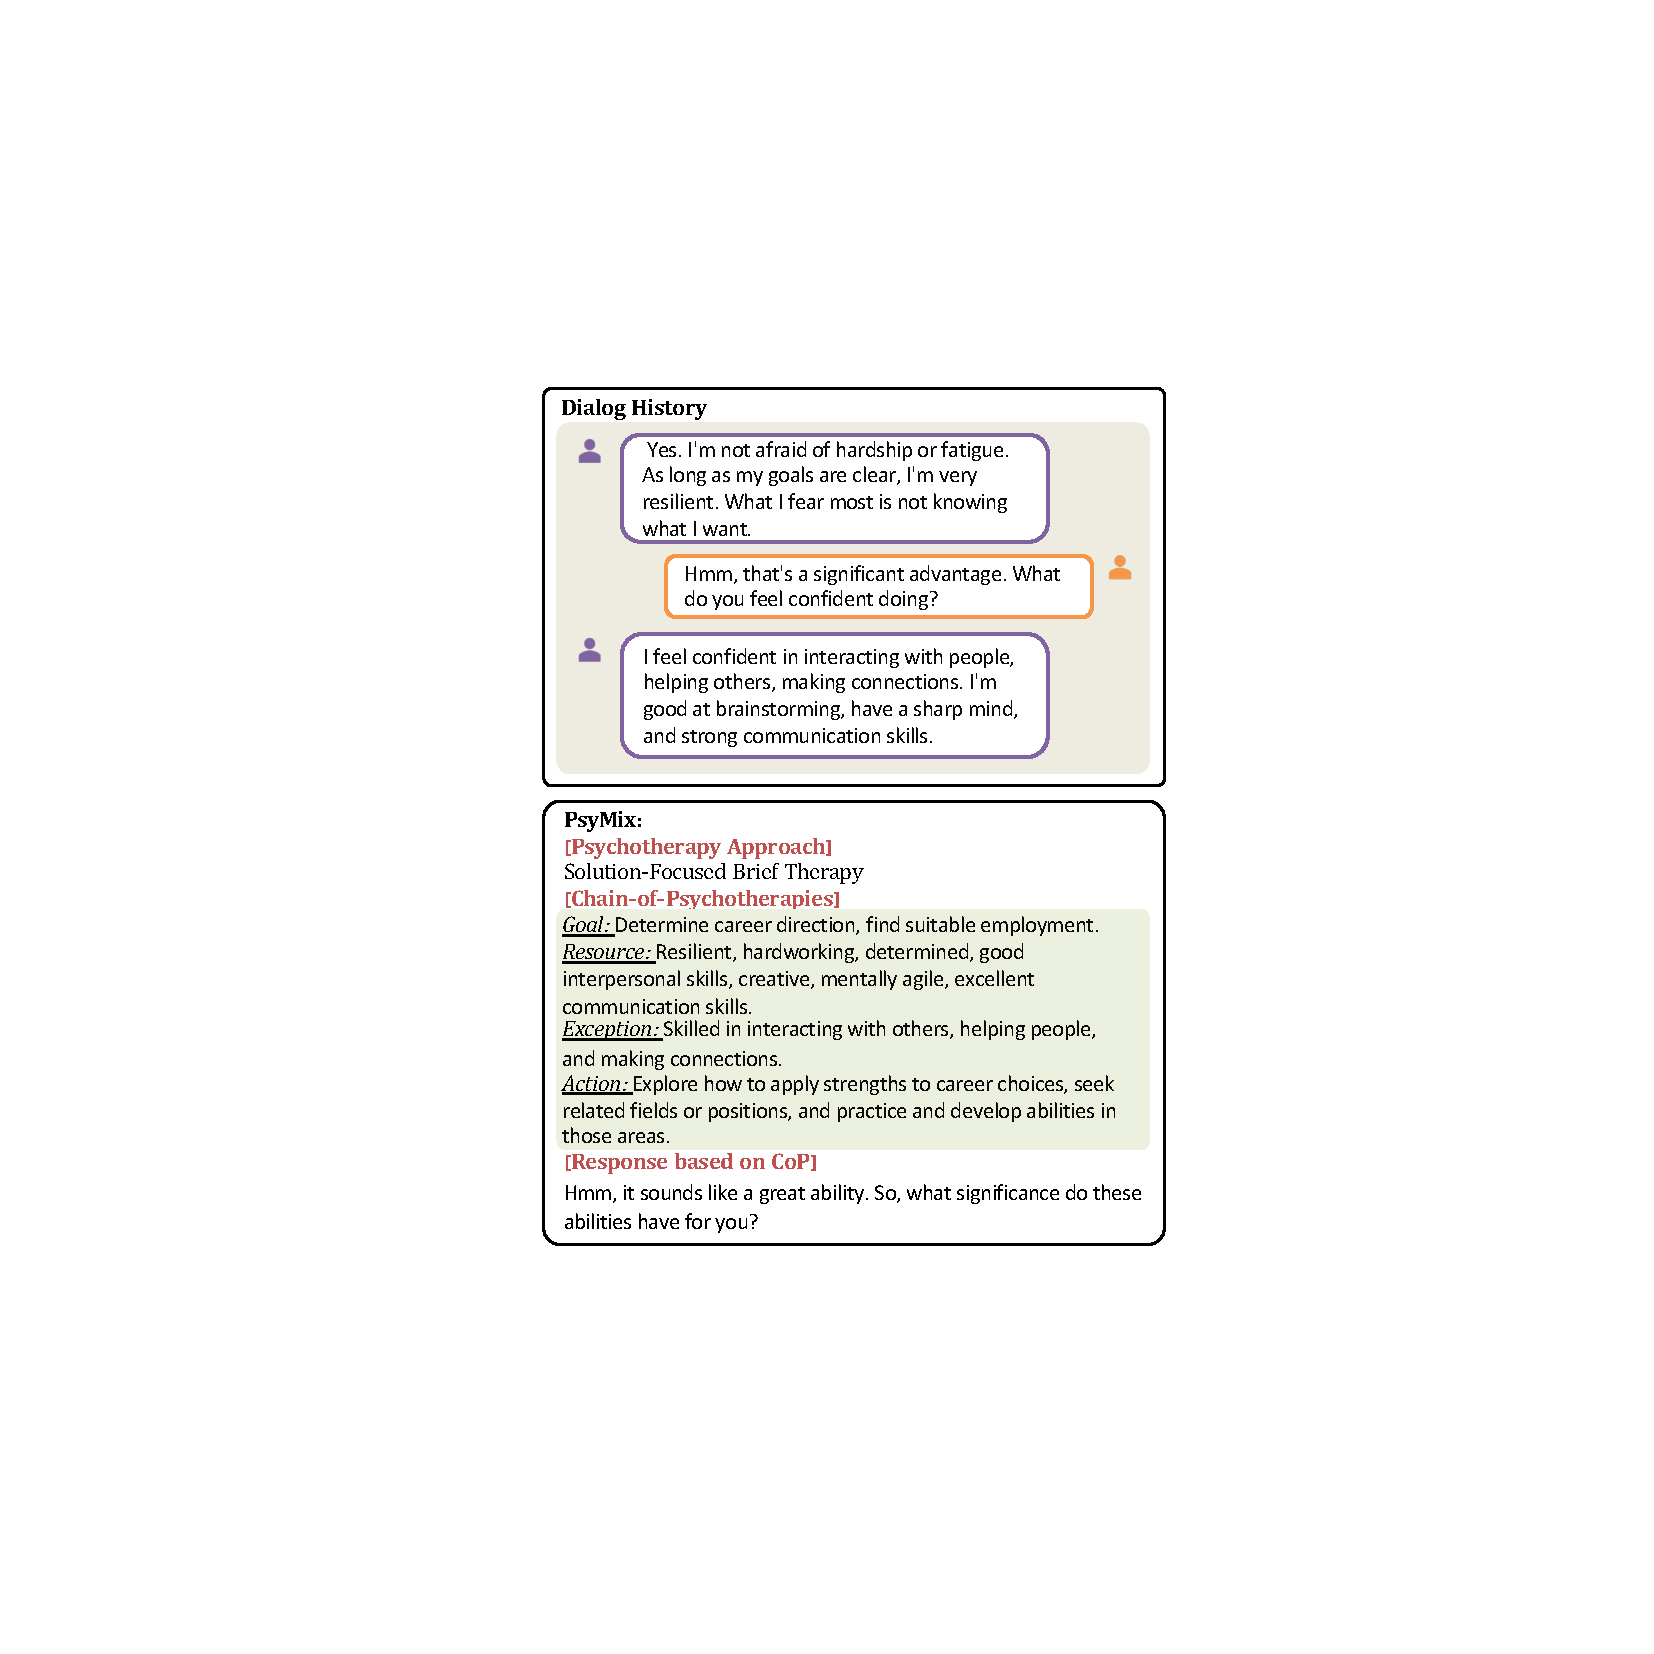
\includegraphics[width=\linewidth]{latex/figures/case1.pdf}
	\caption{Chain-of-Psychotherapies for case 1.}
	\label{fig:case1}
\end{figure}

\begin{figure}[th]
	\centering
	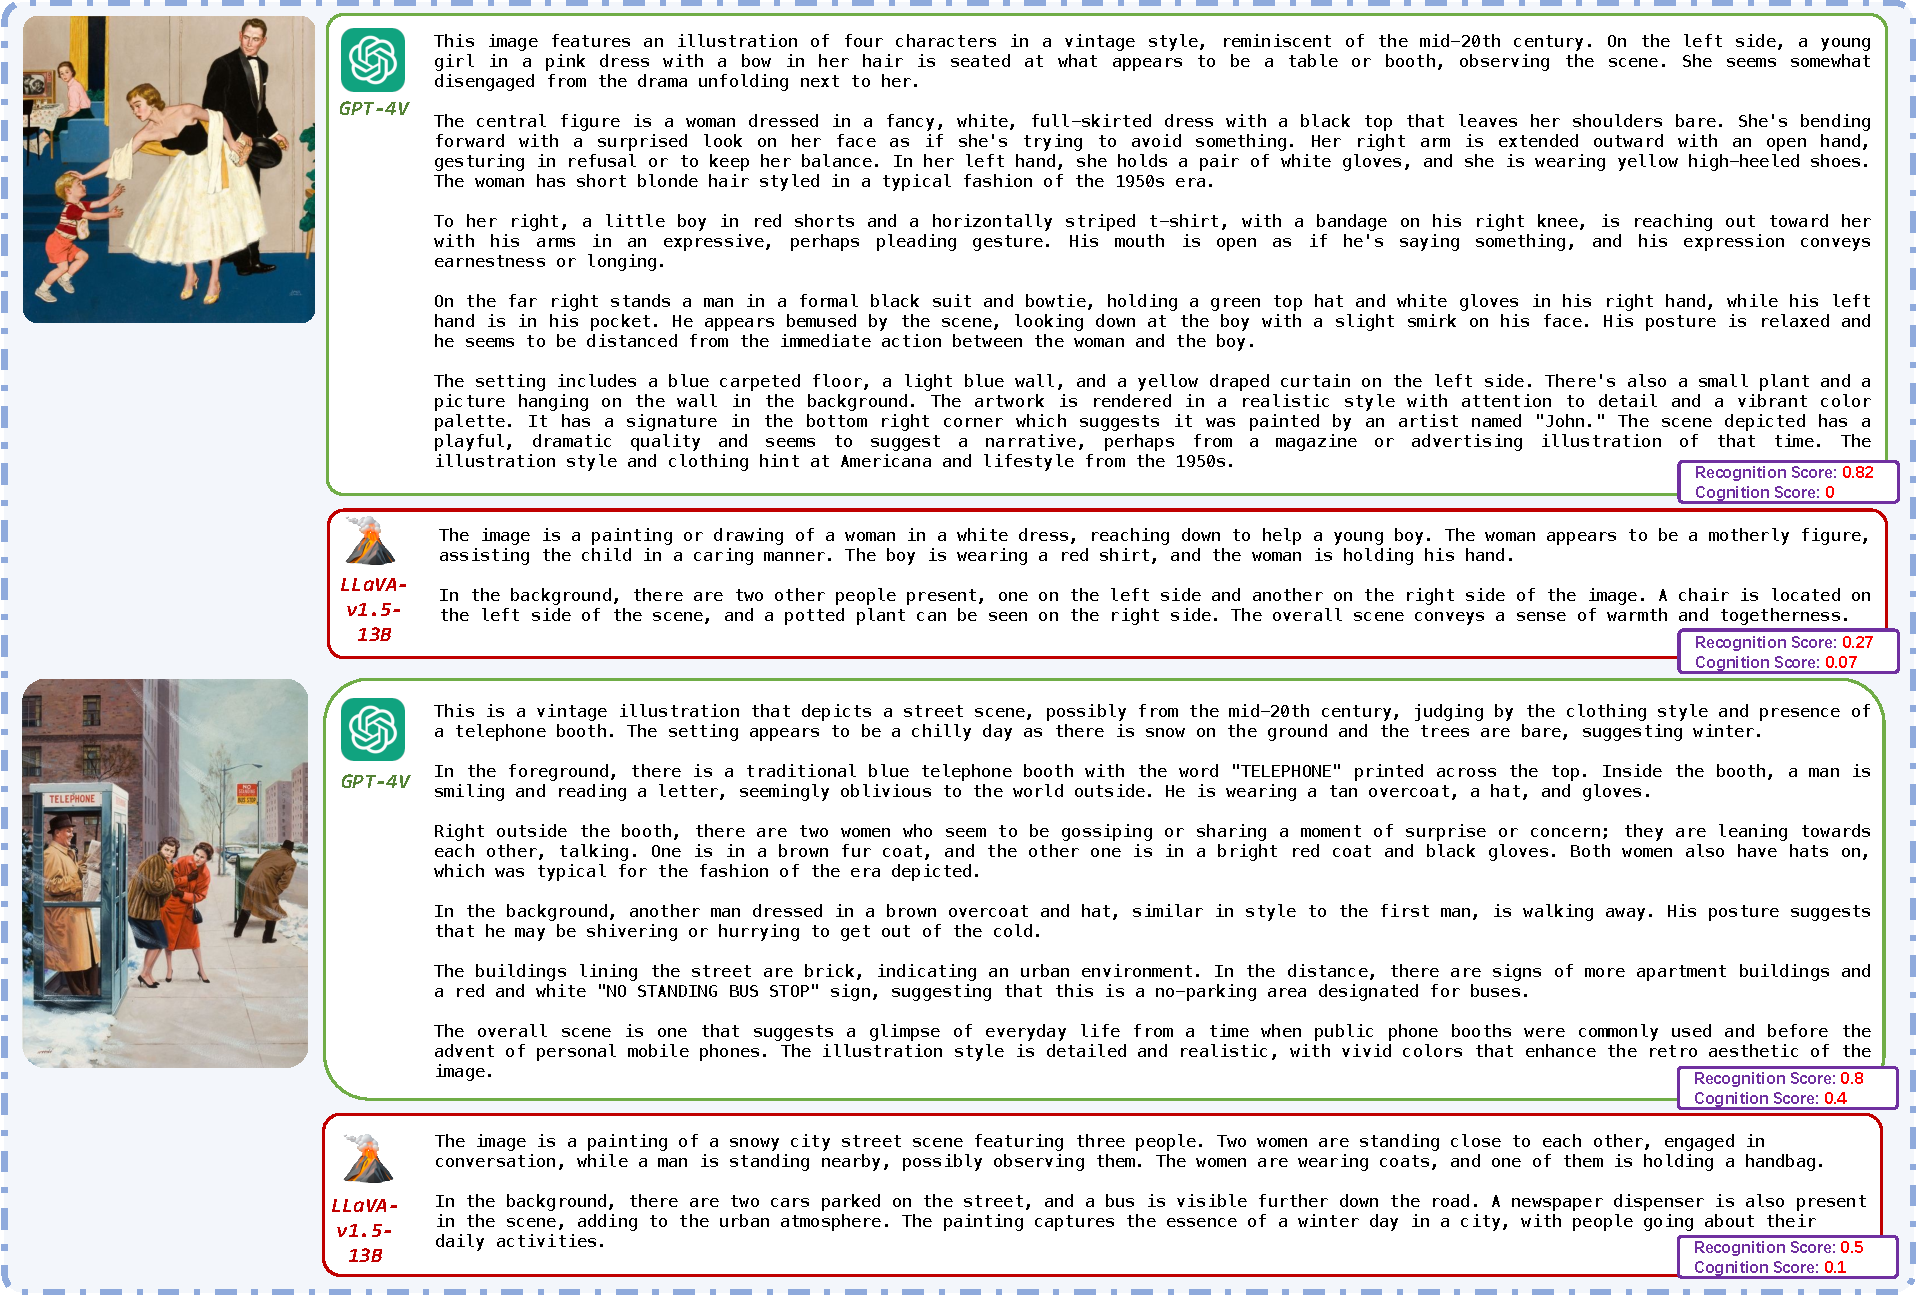
\includegraphics[width=\linewidth]{latex/figures/case2.pdf}
	\caption{Chain-of-Psychotherapies for case 2.}
	\label{fig:case2}
\end{figure}


\begin{figure}[th]
	\centering
	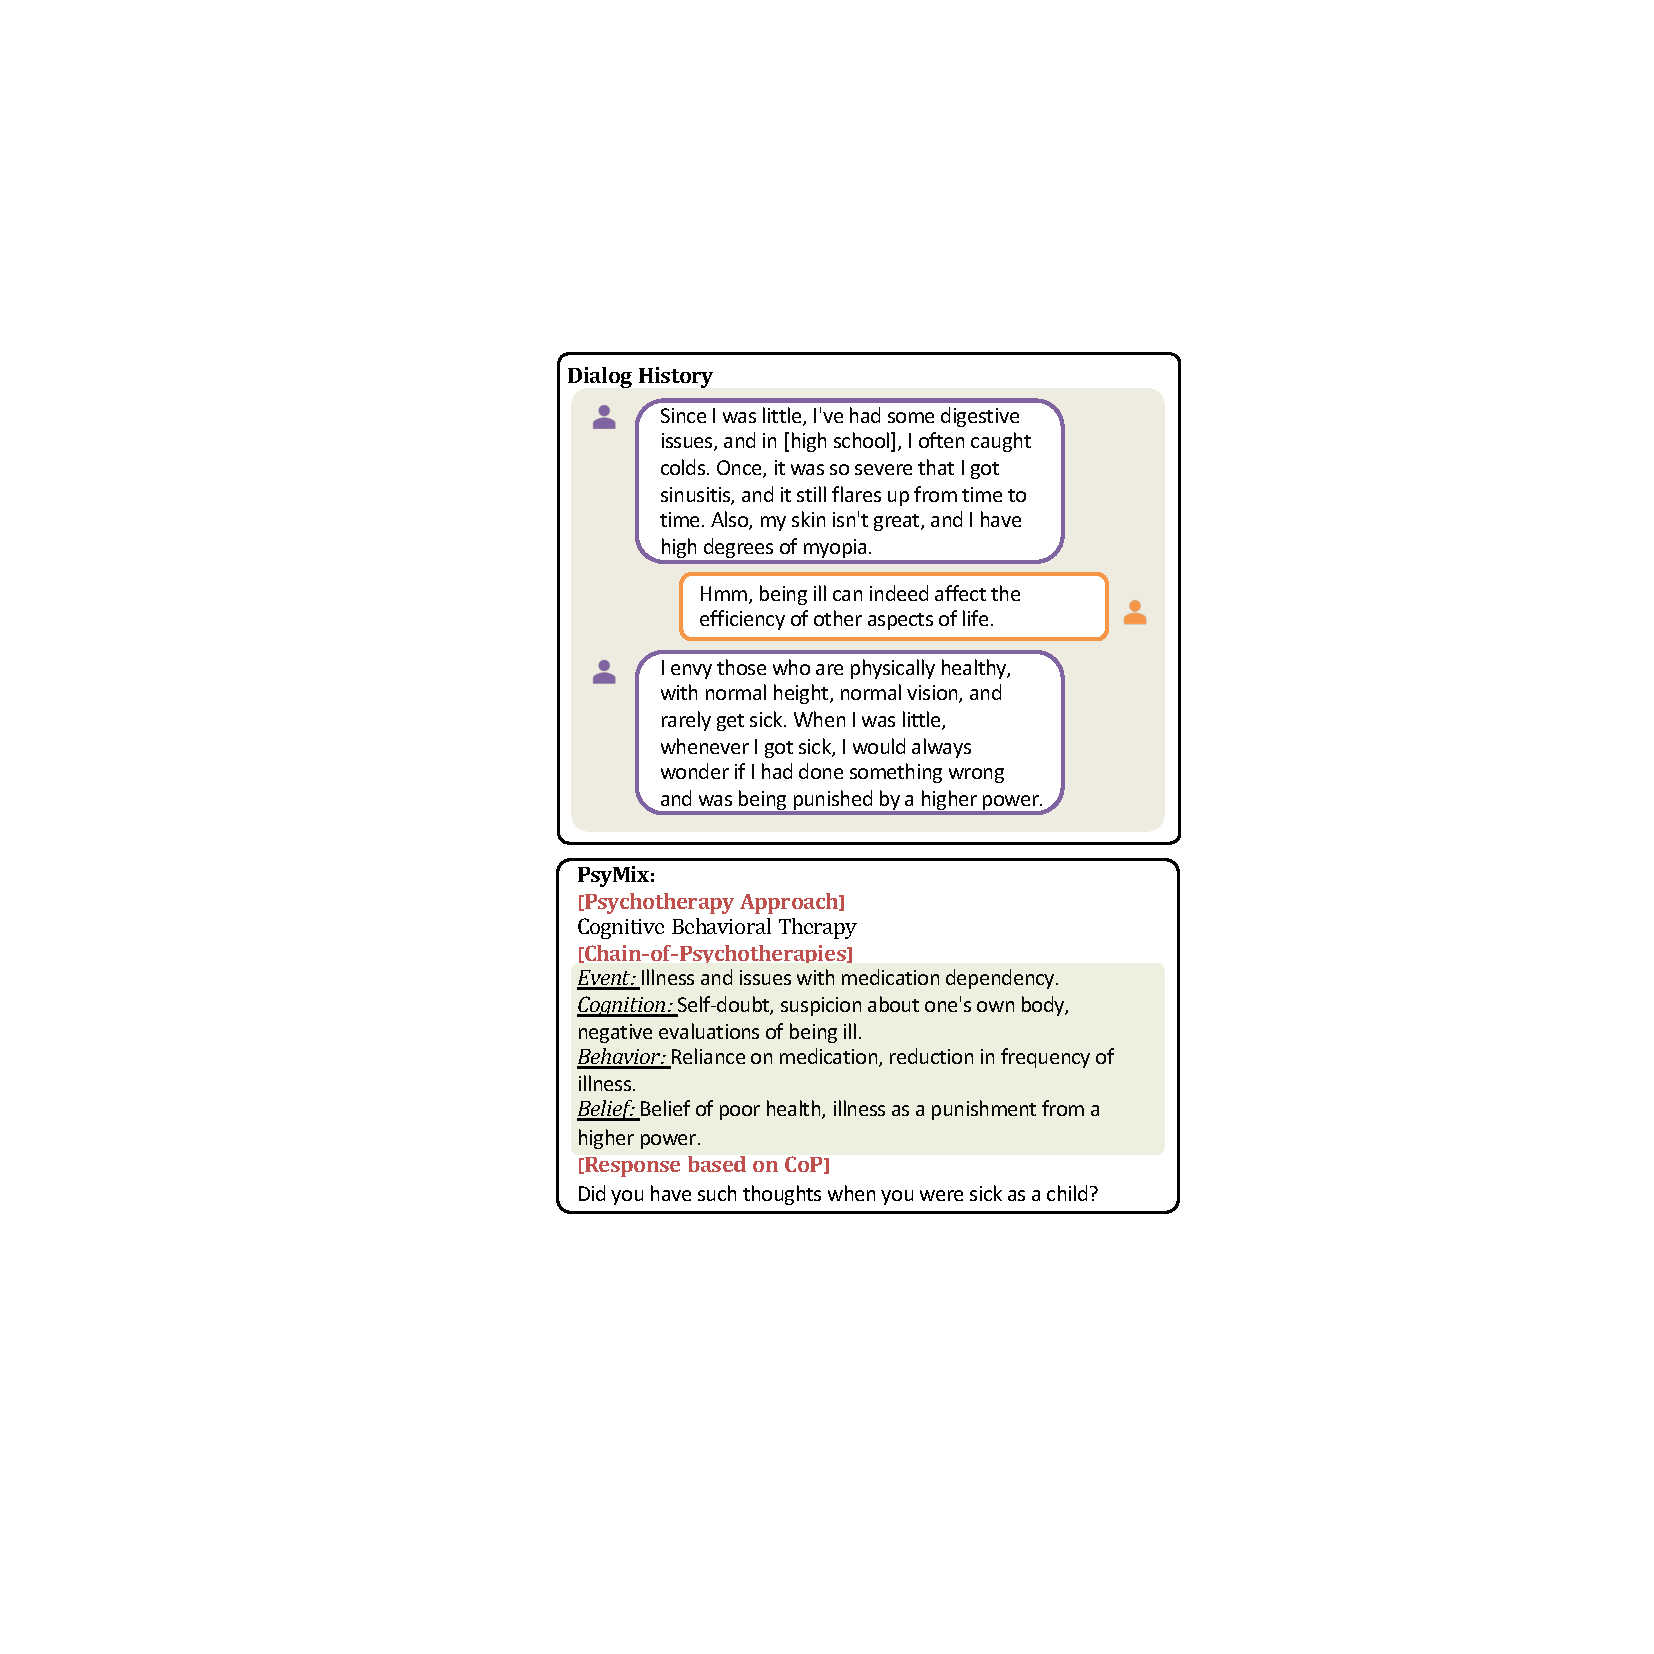
\includegraphics[width=\linewidth]{latex/figures/case3.pdf}
	\caption{Chain-of-Psychotherapies for case 3.}
	\label{fig:case3}
\end{figure}









